\documentclass{article}
\usepackage{v-problem}
\vgeometry

\begin{document}
\vtitle[ROTATION]

\def\pn{01}
\def\exam{JEE}
\def\year{2019}
\def\gdrive{https://drive.google.com/drive/folders/1PEjoi1WM9t8jetcvZErFvZAR9TRcY_9s?usp=share_link}

\def\question{
A circular disc of radius $b$ has a hole of radius $a$ at its centre (see figure). If the mass per unit area of the disc varies as
$\dfrac{\sigma_0}{r}$, then the radius of gyration of the disc about its axis passing through the center is
}

\def\option{
\begin{tasks}(2)
\task $\sqrt{\dfrac{a^2+b^2+ab}{2}}$
\task $\dfrac{a+b}{2}$
\task $\sqrt{\dfrac{a^2+b^2+ab}{3}}$
\task $\dfrac{a+b}{3}$
\end{tasks}
}

\vspace*{\fill}
\begin{tikzpicture}
	\node[qnumber] (n) at (0, 0)[scale=2] {$\pn.$};
	\node[question] (q) [right=2mm of n.east] {\question};
	\tzline[divider]<-0.125, 0> (q.north west)(q.south west);
	\node[format] (f) at  (q.south east){[\exam \quad \year]};
\end{tikzpicture}	
\vspace*{\fill}


\begin{center}
\begin{tikzpicture}
	\tzring*[pattern=crosshatch](0, 0)(1.5)(0, 0)(0.75);
	\tzline[->](0, 0)(25:0.75){$a$}[mb]
	\tzline[->](0, 0)(65:1.5){$b$}[mr]
\end{tikzpicture}
\end{center}
\vspace*{\fill}

\begin{tikzpicture}
\node[minimum width=1cm](n) at (0, 0){}; 
\node[option, anchor=west] at (n.east){\option};
\end{tikzpicture}
\vspace*{\fill}
\pagebreak
\vtitle[\texttt{Solution}]

\begin{center}
\begin{tikzpicture}
	\tzring*[pattern=crosshatch](0, 0)(1.5)(0, 0)(0.75);
	\tzline[->](0, 0)(0:1.05){$r$}[mb]
	\tzline[->](0:1.4)(0:1.2)
	\tznode(0:1.1){$\d{r}$}[b, scale=0.7]
	\tzline[->](0, 0)(65:1.5){$b$}[mr]
	\tzring*[black](0, 0)(1.2)(0, 0)(1.05);
\end{tikzpicture}
\end{center}

\begin{align*}
MK^2 &= I\\
K^2\int_a^b \d{m} &= \int_a^b r^2\d{m}\\
K^2\int_a^b \dfrac{\sigma_0}{r} 2\pi r\d{r} &= \int_a^b r^2\dfrac{\sigma_0}{r} 2\pi r\d{r}\\
K^2\int_a^b \d{r} &= \int_a^b r^2 \d{r}\\
K &= \sqrt{\dfrac{b^3-a^3}{3\left(b-a\right)}}\\
	&=\sqrt{\dfrac{a^2+b^2+ab}{3}} \ans
\end{align*}


\pagebreak

\vspace*{\fill}
\begin{center}
	\fbox{\qrcode[height=2cm]{\gdrive}}
\end{center}
\vspace*{\fill}

\end{document}
